\documentclass[journal,12pt,twocolumn]{IEEEtran}

\usepackage{setspace}
%\usepackage{gensymb}
\singlespacing
\usepackage[cmex10]{amsmath}

\usepackage{amsthm}

\usepackage{mathrsfs}
\usepackage{txfonts}
%\usepackage{stfloats}
\usepackage{bm}
\usepackage{cite}
%\usepackage{cases}
\usepackage{subfig}

\usepackage{longtable}
%\usepackage{multirow}

%\usepackage{enumitem}
\usepackage{mathtools}
%\usepackage{steinmetz}
%\usepackage{tikz}
%\usepackage{circuitikz}
\usepackage{verbatim}
%\usepackage{tfrupee}
\usepackage[breaklinks=true]{hyperref}
\usepackage{graphicx}
%\usepackage{tkz-euclide}

%\usetikzlibrary{calc,math}
\usepackage{listings}
    \usepackage{color}                                            %%
    \usepackage{array}                                            %%
    \usepackage{longtable}                                        %%
    \usepackage{calc}                                             %%
    %\usepackage{multirow}                                         %%
    \usepackage{hhline}                                           %%
    \usepackage{ifthen}                                           %%
    \usepackage{lscape}     
\usepackage{multicol}
%\usepackage{chngcntr}

\DeclareMathOperator*{\Res}{Res}

\renewcommand\thesection{\arabic{section}}
\renewcommand\thesubsection{\thesection.\arabic{subsection}}
\renewcommand\thesubsubsection{\thesubsection.\arabic{subsubsection}}

\renewcommand\thesectiondis{\arabic{section}}
\renewcommand\thesubsectiondis{\thesectiondis.\arabic{subsection}}
\renewcommand\thesubsubsectiondis{\thesubsectiondis.\arabic{subsubsection}}


\hyphenation{op-tical net-works semi-conduc-tor}
\def\inputGnumericTable{}                                 %%

\lstset{
%language=C,
frame=single, 
breaklines=true,
columns=fullflexible
}
\begin{document}


\newtheorem{theorem}{Theorem}[section]
\newtheorem{problem}{Problem}
\newtheorem{proposition}{Proposition}[section]
\newtheorem{lemma}{Lemma}[section]
\newtheorem{corollary}[theorem]{Corollary}
\newtheorem{example}{Example}[section]
\newtheorem{definition}[problem]{Definition}

\newcommand{\BEQA}{\begin{eqnarray}}
\newcommand{\EEQA}{\end{eqnarray}}
\newcommand{\define}{\stackrel{\triangle}{=}}
\bibliographystyle{IEEEtran}
\raggedbottom
\setlength{\parindent}{0pt}
\providecommand{\mbf}{\mathbf}
\providecommand{\pr}[1]{\ensuremath{\Pr\left(#1\right)}}
\providecommand{\qfunc}[1]{\ensuremath{Q\left(#1\right)}}
\providecommand{\sbrak}[1]{\ensuremath{{}\left[#1\right]}}
\providecommand{\lsbrak}[1]{\ensuremath{{}\left[#1\right.}}
\providecommand{\rsbrak}[1]{\ensuremath{{}\left.#1\right]}}
\providecommand{\brak}[1]{\ensuremath{\left(#1\right)}}
\providecommand{\lbrak}[1]{\ensuremath{\left(#1\right.}}
\providecommand{\rbrak}[1]{\ensuremath{\left.#1\right)}}
\providecommand{\cbrak}[1]{\ensuremath{\left\{#1\right\}}}
\providecommand{\lcbrak}[1]{\ensuremath{\left\{#1\right.}}
\providecommand{\rcbrak}[1]{\ensuremath{\left.#1\right\}}}
\theoremstyle{remark}
\newtheorem{rem}{Remark}
\newcommand{\sgn}{\mathop{\mathrm{sgn}}}
\providecommand{\abs}[1]{\left\vert#1\right\vert}
\providecommand{\res}[1]{\Res\displaylimits_{#1}} 
\providecommand{\norm}[1]{\left\lVert#1\right\rVert}
%\providecommand{\norm}[1]{\lVert#1\rVert}
\providecommand{\mtx}[1]{\mathbf{#1}}
\providecommand{\mean}[1]{E\left[ #1 \right]}
\providecommand{\fourier}{\overset{\mathcal{F}}{ \rightleftharpoons}}
%\providecommand{\hilbert}{\overset{\mathcal{H}}{ \rightleftharpoons}}
\providecommand{\system}{\overset{\mathcal{H}}{ \longleftrightarrow}}
	%\newcommand{\solution}[2]{\textbf{Solution:}{#1}}
\newcommand{\solution}{\noindent \textbf{Solution: }}
\newcommand{\cosec}{\,\text{cosec}\,}
\providecommand{\dec}[2]{\ensuremath{\overset{#1}{\underset{#2}{\gtrless}}}}
\newcommand{\myvec}[1]{\ensuremath{\begin{pmatrix}#1\end{pmatrix}}}
\newcommand{\mydet}[1]{\ensuremath{\begin{vmatrix}#1\end{vmatrix}}}
\numberwithin{equation}{subsection}
\makeatletter
\@addtoreset{figure}{problem}
\makeatother
\let\StandardTheFigure\thefigure
\let\vec\mathbf
\renewcommand{\thefigure}{\theproblem}
\def\putbox#1#2#3{\makebox[0in][l]{\makebox[#1][l]{}\raisebox{\baselineskip}[0in][0in]{\raisebox{#2}[0in][0in]{#3}}}}
     \def\rightbox#1{\makebox[0in][r]{#1}}
     \def\centbox#1{\makebox[0in]{#1}}
     \def\topbox#1{\raisebox{-\baselineskip}[0in][0in]{#1}}
     \def\midbox#1{\raisebox{-0.5\baselineskip}[0in][0in]{#1}}
\vspace{3cm}
\title{EE3025 Assignment-1}
\author{Adithya Vardhan - EE18BTECH11008}
\maketitle
\newpage
\bigskip
\renewcommand{\thefigure}{\theenumi}
\renewcommand{\thetable}{\theenumi}
Download all python codes from 
\begin{lstlisting}
https://github.com/Adithya-Vardhan/HW1/tree/main/codes
\end{lstlisting}
%
and latex-tikz codes from 
%
\begin{lstlisting}
https://github.com/Adithya-Vardhan/HW1
\end{lstlisting}
\section{Problem}

Compute 
\begin{align}
	X(k) \triangleq \sum_{n=0}^{N-1} x(n) e^{-j 2 \pi k n / N}, \quad k=0,1, \ldots, N-1
\end{align}\\
and $H(k)$ using h(n).

\section{Solution}
Let
\begin{align}
    x(n) = \cbrak{\underset{\uparrow}{1},2,3,4,2,1} 
\end{align}\\
and the given difference equation is \\
\begin{align}
    y(n) + \frac{1}{2}y(n-1) = x(n) + x(n-2)
\end{align}
By applying Z-transform to the above equation we get, \\
\begin{align}
Y(z) + \frac{1}{2}z^{-1}Y(z)=X(z) + z^{-2}X(z)\\
Y(z)=\frac{2(z^2+1)}{z(2z+1)}X(z)
\end{align}\\
Therefore H(z) is \\
\begin{align}
H(z) = \frac{2(z^2+1)}{z(2z+1)} 
\end{align}
\begin{align}
H(z) &= \frac{1+z^{-2}}{1+\frac{1}{2}z^{-1}}\\
H(z) &= z^{-1}\sbrak{\frac{1}{1+\frac{1}{2}z^{-1}} + \frac{z^{-2}}{1+\frac{1}{2}z^{-1}}}
\end{align}\\
By applying inverse z-transform we get,\\
\begin{align}
    h(n)=\sbrak{\frac{-1}{2}}^nu(n) + \sbrak{\frac{-1}{2}}^{n-2}u(n-2)
\end{align}\\
By using equation 1.0.1 \\
\begin{align}
    X(k) = \sum_{n=0}^{N-1} x(n) e^{-j 2 \pi k n / N}, \quad k=0,1, \ldots, N-1
\end{align}\\
the above equation can be written as,where  $W = e^{\frac{-j2\pi}{N}}$ \\
\begin{align}
\begin{pmatrix}
X(0)\\
X(1)\\
X(2)\\
\vdots\\
X(N-1)
\end{pmatrix}
= 
\begin{pmatrix}
1 & 1 & \cdots & 1 \\
1 & W  &  \cdots & W^{N-1} \\
1 & W^{2} &  \cdots & W^{2(N-1)} \\
\vdots  & \vdots  & \ddots & \vdots  \\
1 & W^{N-1}  &  \cdots & W^{(N-1)(N-1)} \\ 
\end{pmatrix}
\quad
\begin{pmatrix}
x(0)\\
x(1)\\
x(2)\\
\vdots\\
x(N-1)
\end{pmatrix}
\end{align}\\
and \\
\begin{align}
    H(k) = \sum_{n=0}^{N-1} h(n) e^{-j 2 \pi k n / N}, \quad k=0,1, \ldots, N-1
\end{align}\\
the above equation can be written as,
\begin{align}
\begin{pmatrix}
H(0)\\
H(1)\\
H(2)\\
\vdots\\
H(N-1)
\end{pmatrix}
= 
\begin{pmatrix}
1 & 1 & \cdots & 1 \\
1 & W  &  \cdots & W^{N-1} \\
1 & W^{2}  &  \cdots & W^{2(N-1)} \\
\vdots  & \vdots   & \ddots & \vdots  \\
1 & W^{N-1} &  \cdots & W^{(N-1)(N-1)} \\ 
\end{pmatrix}
\quad
\begin{pmatrix}
h(0)\\
h(1)\\
h(2)\\
\vdots\\
h(N-1)
\end{pmatrix}
\end{align}
\newpage
from above mentioned python codes we get  the following plots\\
\begin{figure}[h!]
    \centering
    \includegraphics[width=8cm]{./figures/abs_X(k).eps}
    \caption{Magnitude of X(k)}
    \label{|X(k)|}
\end{figure} \\
\begin{figure}[h!]
    \centering
    \includegraphics[width=8cm]{./figures/angle_X(k).eps}
    \caption{Phase of X(k)}
    \label{/_X(k)}
\end{figure}
\begin{figure}[h!]
    \centering
    \includegraphics[width=8cm]{./figures/abs_h(k).eps}
    \caption{Magnitude of h(k)}
    \label{|h(k)|}
\end{figure} 
\newpage
\begin{figure}[h!]
    \centering
    \includegraphics[width=8cm]{./figures/angle_h(k).eps}
    \caption{Phase of h(k)}
    \label{/_X(k)}
\end{figure} 


consider
\begin{align}
    x(n) = \cbrak{\underset{\uparrow}{1},2,3,4,4,3,2,1} 
\end{align}\\
Let $F_{N}$ be the N-point DFT Matrix. \\
Using the property of Complex Exponentials we can express $F_{N}$ in terms of $F_{N/2}$\\
\begin{equation}
F_{N}=
\begin{bmatrix}
I_{N/2} & D_{N/2} \\
I_{N/2} & -D_{N/2}
\end{bmatrix}
\begin{bmatrix}
F_{N/2} & 0 \\
0 & F_{N/2}
\end{bmatrix}
P_{N}
\end{equation}
For N = 8
\begin{equation}
\implies F_{8}=
\begin{bmatrix}
I_{4} & D_{4} \\
I_{4} & -D_{4}
\end{bmatrix}
\begin{bmatrix}
F_{4} & 0 \\
0 & F_{4}
\end{bmatrix}
P_{8}
\end{equation}
where
$I_{4}$ is the 4x4 identity matrix
\begin{equation}
D_{4}=
\begin{bmatrix}
1 & 0 & 0 & 0\\
0 & W^{1}_{4} & 0 & 0\\
0 & 0 & W^{2}_{4} & 0\\
0 & 0 & 0 & W^{3}_{4}
\end{bmatrix}
\end{equation}
\begin{equation}
P_{8} =
\begin{bmatrix}
1 & 0 & 0 & 0 & 0 & 0 & 0 & 0\\
0 & 0 & 1 & 0 & 0 & 0 & 0 & 0\\
0 & 0 & 0 & 0 & 1 & 0 & 0 & 0\\
0 & 0 & 0 & 0 & 0 & 0 & 1 & 0\\
0 & 1 & 0 & 0 & 0 & 0 & 0 & 0\\
0 & 0 & 0 & 1 & 0 & 0 & 0 & 0\\
0 & 0 & 0 & 0 & 0 & 1 & 0 & 0\\
0 & 0 & 0 & 0 & 0 & 0 & 0 & 1

\end{bmatrix} 
\end{equation}\\
Step by Step visualization of computing 8-Point DFT recursively using 4-point DFT's and 2-point DFT's.Expressing 8-point DFT's in terms of 4-point DFT's.
\begin{equation}
\begin{bmatrix}
X(0) \\ 
X(1) \\ 
X(2) \\ 
X(3)
\end{bmatrix}
=
\begin{bmatrix}
X_{e}(0) \\ 
X_{e}(1)\\ 
X_{e}(2)\\
X_{e}(3)\\
\end{bmatrix}
+
\begin{bmatrix}
W^{0}_{8} & 0 & 0 & 0\\
0 & W^{1}_{8} & 0 & 0\\
0 & 0 & W^{2}_{8} & 0\\
0 & 0 & 0 & W^{3}_{8}
\end{bmatrix}
\begin{bmatrix}
X_{o}(0) \\ 
X_{o}(1) \\ 
X_{o}(2) \\
X_{o}(3)
\end{bmatrix}
\end{equation}
\begin{equation}
\begin{bmatrix}
X(4) \\ 
X(5) \\ 
X(6) \\ 
X(7)
\end{bmatrix}
=
\begin{bmatrix}
X_{e}(0) \\ 
X_{e}(1)\\ 
X_{e}(2)\\
X_{e}(3)\\
\end{bmatrix}
-
\begin{bmatrix}
W^{0}_{8} & 0 & 0 & 0\\
0 & W^{1}_{8} & 0 & 0\\
0 & 0 & W^{2}_{8} & 0\\
0 & 0 & 0 & W^{3}_{8}
\end{bmatrix}
\begin{bmatrix}
X_{o}(0) \\ 
X_{o}(1) \\ 
X_{o}(2) \\
X_{o}(3)
\end{bmatrix}
\end{equation}
Now, 4-point DFT's to 2-point DFT's
\begin{equation}
\begin{bmatrix}
X_{e}(0) \\ 
X_{e}(1)\\ 
\end{bmatrix}
=
\begin{bmatrix}
X_{e_{1}}(0) \\ 
X_{e_{1}}(1)\\ 
\end{bmatrix}
+
\begin{bmatrix}
W^{0}_{4} & 0\\
0 & W^{1}_{4}
\end{bmatrix}
\begin{bmatrix}
X_{o_{1}}(0) \\ 
X_{o_{1}}(1) \\ 
\end{bmatrix}
\end{equation}
\begin{equation}
\begin{bmatrix}
X_{e}(2) \\ 
X_{e}(3)\\ 
\end{bmatrix}
=
\begin{bmatrix}
X_{e_{1}}(0) \\ 
X_{e_{1}}(1)\\ 
\end{bmatrix}
-
\begin{bmatrix}
W^{0}_{4} & 0\\
0 & W^{1}_{4}
\end{bmatrix}
\begin{bmatrix}
X_{o_{1}}(0) \\ 
X_{o_{1}}(1) \\ 
\end{bmatrix}
\end{equation}
\begin{equation}
\begin{bmatrix}
X_{o}(0) \\ 
X_{o}(1)\\ 
\end{bmatrix}
=
\begin{bmatrix}
X_{e_{2}}(0) \\ 
X_{e_{2}}(1)\\ 
\end{bmatrix}
+
\begin{bmatrix}
W^{0}_{4} & 0\\
0 & W^{1}_{4}
\end{bmatrix}
\begin{bmatrix}
X_{o_{2}}(0) \\ 
X_{o_{2}}(1) \\ 
\end{bmatrix}
\end{equation}
\begin{equation}
\begin{bmatrix}
X_{o}(2) \\ 
X_{o}(3)\\ 
\end{bmatrix}
=
\begin{bmatrix}
X_{e_{2}}(0) \\ 
X_{e_{2}}(1)\\ 
\end{bmatrix}
-
\begin{bmatrix}
W^{0}_{4} & 0\\
0 & W^{1}_{4}
\end{bmatrix}
\begin{bmatrix}
X_{o_{2}}(0) \\ 
X_{o_{2}}(1) \\ 
\end{bmatrix}
\end{equation}
\begin{equation}
P_{8}
\begin{bmatrix}
x(0) \\ 
x(1) \\ 
x(2) \\ 
x(3) \\ 
x(4) \\ 
x(5) \\
x(6) \\
x(7)
\end{bmatrix}
 = 
\begin{bmatrix}
x(0) \\ 
x(2) \\ 
x(4) \\ 
x(6) \\
x(1) \\ 
x(3) \\ 
x(5) \\
x(7)
\end{bmatrix}
\end{equation}
\begin{equation}
P_{4}
\begin{bmatrix}
x(0) \\ 
x(2) \\ 
x(4) \\ 
x(6) \\
\end{bmatrix}
 = 
\begin{bmatrix}
x(0) \\ 
x(4) \\ 
x(2) \\
x(6)
\end{bmatrix}
\end{equation}
\begin{equation}
P_{4}
\begin{bmatrix}
x(1) \\ 
x(3) \\ 
x(5) \\
x(7)
\end{bmatrix}
 = 
\begin{bmatrix}
x(1) \\ 
x(5) \\ 
x(3) \\ 
x(7) \\
\end{bmatrix}
\end{equation}
Finally,
\begin{equation}
\begin{bmatrix}
X_{e_{1}}(0) \\ 
X_{e_{1}}(1)\\ 
\end{bmatrix}
= F_{2}
\begin{bmatrix}
x(0) \\ 
x(4) \\ 
\end{bmatrix}
=
\begin{bmatrix}
x(0)+x(4) \\ 
x(0)-x(4) \\ 
\end{bmatrix}
\end{equation}
\begin{equation}
\begin{bmatrix}
X_{o_{1}}(0) \\ 
X_{o_{1}}(1)\\ 
\end{bmatrix}
= F_{2}
\begin{bmatrix}
x(2) \\ 
x(6) \\ 
\end{bmatrix}
=
\begin{bmatrix}
x(2)+x(6) \\ 
x(2)-x(6) \\ 
\end{bmatrix}
\end{equation}
\begin{equation}
\begin{bmatrix}
X_{e_{2}}(0) \\ 
X_{e_{2}}(1)\\ 
\end{bmatrix}
= F_{2}
\begin{bmatrix}
x(1) \\ 
x(5) \\ 
\end{bmatrix}
=
\begin{bmatrix}
x(1)+x(5) \\ 
x(1)-x(5) \\ 
\end{bmatrix}
\end{equation}
\begin{equation}
\begin{bmatrix}
X_{o_{2}}(0) \\ 
X_{o_{2}}(1)\\ 
\end{bmatrix}
= F_{2}
\begin{bmatrix}
x(3) \\ 
x(7) \\ 
\end{bmatrix}
=
\begin{bmatrix}
x(3)+x(7) \\ 
x(3)-x(7) \\ 
\end{bmatrix}
\end{equation}
So, $X_{e_{2}} \in \text{DFT} \{x(1),x(5)\}$ and $X_{o_{2}} \in \text{DFT} \{x(3),x(7)\}$ would combine to give $X_{o}$ .And $X_{e_{1}} \in \text{DFT} \{x(0),x(4)\}$ and $X_{o_{1}} \in \text{DFT} \{x(2),x(6)\}$ would combine to give $X_{e}$.

from above mentioned python codes we get  the following plots\\
\begin{lstlisting}
https://github.com/Adithya-Vardhan/HW1/tree/main/codes
\end{lstlisting}

\begin{figure}[h!]
    \centering
    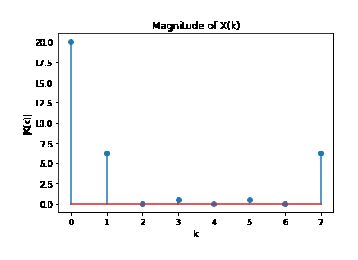
\includegraphics[width=8cm]{./figures/abs_x(k)_2.eps}
    \caption{Magnitude of x(k)}
    \label{|h(k)|}
\end{figure} 
\begin{figure}[h!]
    \centering
    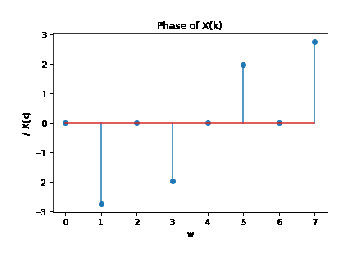
\includegraphics[width=8cm]{./figures/phase_x(k)_2.eps}
    \caption{Phase of x(k)}
    \label{/_X(k)}
\end{figure} 
\end{document}  

